% introduzione al corso di codifica del testo anno accademico 2018/2019

\documentclass{beamer}
    
%    \usepackage[english]{babel}
    %\usepackage[latin1]{inputenc}
    %\usepackage[T1]{fontenc}

\mode<presentation>{
  \setbeamertemplate{background canvas}[vertical shading]
  \usetheme{Berkeley}
  \useoutertheme{himinfolines}
}
  
\usepackage{ucs}
\usepackage[utf8]{inputenc}
\usepackage[english,polutonikogreek,italian,UKenglish,british]{babel}
\usepackage{graphicx}
\usepackage{colortbl}
\usepackage{multicol}
\usepackage{ulem}
\usepackage{verbatim}
\usepackage{alltt}
\usepackage{ccicons}
\usepackage{MnSymbol,wasysym}
\usepackage{tikzsymbols}
\usepackage{textcomp}
\usepackage{xmpincl}

\usepackage{parskip}
\setcounter{nframes}{70}
\setcounter{nframe}{1}
\setbeamercovered{dynamic}
\newenvironment{grcenv}{\begin{otherlanguage}{greek}}{\end{otherlanguage}}
\newcommand{\g}[1]{\textgreek{#1}}
\definecolor{darkgreen}{rgb}{0,0.5,0}
\definecolor{darkblue}{rgb}{0,0,0.5}
\definecolor{grey}{rgb}{0.5,0.5,0.5}
\setcounter{tocdepth}{5}

\makeatletter

\makeatother
%\includexmp{LicencesAndLicensing}

%frame00 metadata
    \title{Presentazione del Corso Codifica di Testi \\a.a. 2018-2019}
    \author[A.M. Del Grosso]{Angelo Mario Del Grosso}
    %\institute{\texttt{angelo.delgrosso@ilc.cnr.it} \\\bigskip\textit{CNR-ILC-LicoLab} \\\bigskip\url{http://licolab.ilc.cnr.it/}}
    \institute{\texttt{angelo.delgrosso@ilc.cnr.it} \\\bigskip\textit{CNR-ILC-LicoLab}}
    \date{Istituto di Linguistica Computazionale ``A. Zampolli'', \today}
    \AtBeginSection[]{
    \begin{frame}<beamer>
    \addtocounter{nframe}{1}
    \footnotesize
    \frametitle{Progress status}
    \tableofcontents[currentsection,hideothersubsections]
    \end{frame}
    }

\begin{document}

\begin{frame}
	\maketitle
\end{frame}

\begin{frame}
	\frametitle{Piano della presentazione}
	\tableofcontents
\end{frame}

\section{Presentazione}

\begin{frame}
	\frametitle{Di cosa mi occupo}
	\addtocounter{nframe}{1}

	\begin{block}{Filologia Computazionale}
		%slide di presentazione: chi sono, piccola bio, di cosa mi occupo
		%\\prendere dal curriculum alcuni pezzi mettere mail istituzionale ed eventualmente telefono
		Analisi, progettazione e sviluppo di componenti software per sistemi Web di linguistica e filologia digitale/computazionale volti al trattamento di testi di tradizione medievale, a stampa e di autori moderni e contemporanei.
	\end{block}

	\begin{block}{Modelli Object Oriented per il Textual Scholarship}
		Impiego delle nuove tecnologie nell’ambito delle Digital Humanities (DH) per la progettazione
		object–oriented di strumenti digitali Web–based rispondenti alle esigenze degli utenti accademici, studenti e sviluppatori.
	\end{block}




\end{frame}

\begin{frame}
	\frametitle{Presentazione del Corso}
	\addtocounter{nframe}{1}

	\begin{center}
		
\includegraphics[width=.5\textwidth]{../imgs/tei-r.pdf}
	\end{center}

	%\begin{itemize}
	%	\item<1-> Introduzione
	%	\item<2-> Codifica dei Caratteri
	%   \item<3-> Codifica dei Testi
	%   \item<4-> Ecosistema XML (Linee Guida TEI)
	%   \item<5-> Conclusioni
	%\end{itemize}

\end{frame}



\section{Introduzione}

% sezione intro frame 01
\begin{frame}
    \frametitle{Introduzione al Corso di Codifica di Testi}
    \framesubtitle{Obiettivi, competenze e conoscenze}
    \addtocounter{nframe}{1}
    
    \begin{block}{Obiettivo}
        Illustrare i principi di modellazione e le prassi di codifica del testo per una adeguata rappresentazione ed elaborazione digitale di risorse testuali.  
    \end{block}

    \begin{block}{Rationale}
       Fornire gli strumenti e le conoscenze necessarie per progettare e realizzare criticamente una codifica digitale di testi complessi, in particolare testi letterari e di interesse storico-culturale, usando le linee guida della Text Encoding Initiative (TEI).
    \end{block}

\end{frame}

% sezione intro frame 02
\begin{frame}
    \frametitle{Argomenti trattati}
    \framesubtitle{Obiettivi, competenze e conoscenze}
    \addtocounter{nframe}{1}
    
    \begin{block}{Competenze attese}
        Al termine del corso sarete in grado di valutare il metodo di codifica più appropriato allo scenario d'interesse, di creare uno schema di codifica TEI e di usare gli strumenti più idonei per la codifica e la (semplice) elaborazione e visualizzazione di un testo.
    \end{block}

\end{frame}

% sezione intro frame 03
\begin{frame}
    \frametitle{Principali Argomenti}
    \framesubtitle{Obiettivi, competenze e conoscenze}
    \addtocounter{nframe}{1}

    
        \begin{itemize}
            \item Codifica dei caratteri e di testi
            \item I linguaggi di markup e introduzione a XML
            \item Creazione di schemi di codifica
            \item Le norme TEI (Text Encoding Initiative)
            \item Alcuni specifici Moduli TEI
            \item Definizione di schemi di codifica personalizzati
            \item introduzione ai fogli di stile XSLT
            \item elaborazione documenti XML-TEI (XSLT2.0, DOM)
            \item esempi, esercitazioni e seminari 
        \end{itemize}

\end{frame}

\begin{frame}
    \frametitle{Bozza piano del Corso: Calendario 2018/2019}
    \framesubtitle{Lunedì dalle 14.00 alle 18.00}
    \addtocounter{nframe}{1}
    
        \begin{itemize}
            \setlength\itemsep{0.5em}
            \item Lezione 1 (24/9): Introduzione al corso e strumenti software utilizzati
            \item Lezione 2 (1/10): Elementi teorici relativi alla rappresentazione del testo
            \item Lezione 3 (8/10) Elementi di XML e introduzione alla definizione degli Schemi XML
            \item Lezione 4 (15/10): Elementi di Codifica TEI
            \item Lezione 5 (22/10): Modulo Specifico TEI
        \end{itemize}

\end{frame}

\begin{frame}
    \frametitle{Bozza piano del Corso: Calendario 2018/2019}
    \framesubtitle{Lunedì dalle 14.00 alle 18.00}
    \addtocounter{nframe}{1}
    
        \begin{itemize}
            \setlength\itemsep{0.5em}
            \item Lezione 6 (29/10): Moduli Editoriali TEI
            \item Lezione 7 (5/11): Codifica dei caratteri e Unicode
            \item Lezione 8 (12/11): Elaborazione documenti XML-TEI (XSLT e DOM)
            \item Lezione 9 (19/11): Esercitazione e discussione sui progetti 
            \item Lezione 10 (26/11): Esercitazione e Recupero Argomenti
            \item (03/12-17/12):  Eventuali esercitazioni, attività laboratoriali, recupero argomenti
        \end{itemize}

\end{frame}

% sezione intro frame 04
\begin{frame}
    \frametitle{Perché è importante la codifica dei testi}
    \framesubtitle{Motivazioni pratiche}
    \addtocounter{nframe}{1}
    
    \begin{block}{Dove troviamo i testi}
        Nella nostra cultura tradizionale la quasi totalità dei testi è ``registrata'', ``trasmessa'' e quindi ``conservata'' attraverso supporti e materiali fisici di varia natura e forma (iscrizioni su pietra, manoscritti di pergamena, papiri, carta, libri a stampa, incunabula, cinquecentine, etc).
    \end{block}

\end{frame}

% sezione intro frame 05
\begin{frame}
    \frametitle{Perché è importante la codifica dei testi}
    \framesubtitle{Motivazioni pratiche}
    \addtocounter{nframe}{1}
    
    \begin{block}{Perché codificare i testi}
        Per rendere disponibile questo patrimonio attraverso i sistemi per la gestione dell'informazione digitali e computazionali è necessario effettuare una trasposizione/transcodifica\textsuperscript{*} dei testi dal loro supporto originario verso il nuovo supporto elettronico.
    \end{block}

    \begin{center}
        * \textit{procedimento di conversione dei dati codificati secondo un sistema verso un sistema diverso}
    \end{center}

\end{frame}

% sezione intro frame 06
\begin{frame}
    \frametitle{Perché è importante la codifica dei testi}
    \framesubtitle{Motivazioni teoriche}
    \addtocounter{nframe}{1}
    
    \begin{block}{Scienze umane vs Scienze informatiche}
        Il rapporto tra sapere umanistico e informatica non è solo una questione meramente strumentale:\\ 
        \textit{l'informatica non è solo un utensile dalle notevoli capacità.}

        \begin{center}
            Salto di paradigma sia da un punto di vista teorico sia metodologico.
        \end{center} 
    \end{block}

\end{frame}

%sezione intro frame 06b
\begin{frame}
    \frametitle{Perché è importante la codifica dei testi}
    \framesubtitle{Motivazioni teoriche}
    \addtocounter{nframe}{1}
    
    \begin{block}{La codifica come metodologia}
        L'attività di codifica diviene funzione metodologica nell'ambito delle discipline che si occupano del testo.
     \end{block}

     \begin{block}{La codifica come analisi teorica}
     Il linguaggio di codifica adottato può essere considerato come un linguaggio teorico:
      
     \begin{center}
        \textit{Esplicitare e formalizzare le ipotesi interpretative su un certo oggetto di studio}
     \end{center} 
    \end{block}

\end{frame}

% sezione intro frame 07
\begin{frame}
    \frametitle{Perché è importante la codifica dei testi}
    \framesubtitle{In sintesi}
    \addtocounter{nframe}{1}
    
    \begin{block}{Rappresentare il testo}
         Il focus del corso sarà incentrato sulla rappresentazione digitale del testo.
    \end{block}

    \begin{block}{Esistono dibattiti e controversie}
        Per ottenere una rappresentazione digitale del testo ci sono diversi formati e formalismi:
        \\ la nostra scelta ricade sulle norme suggerite dal consorzio TEI.
    
        Molte questioni ancora non sono state risolte altre sono molto controverse, sia teorico-metodologico, sia pratico-tecnologico.
   
    \end{block}

\end{frame}

% sezione intro frame 08
\begin{frame}
    \frametitle{Perché è importante la codifica dei testi}
    \framesubtitle{Ma in definitiva}
    \addtocounter{nframe}{1}
    
    \begin{block}{Perché codificare}

        \begin{center}
            \textit{Le differenze di formato sono più che altro estetiche e non sostanziali}
        \end{center}

    \end{block}
     

    \begin{block}{Perché codificare}

        \begin{center}
            \textbf{Ma anche l'occhio \underline{umano} vuole la sua parte}
        \end{center}
       
    \end{block}

\end{frame}



\section{Codifica dei Caratteri}
% frame 00
\begin{frame}
	\frametitle{Elementi di Codifica dei Caratteri}
	\framesubtitle{Definizioni}
	\addtocounter{nframe}{1}

	\begin{block}{Rappresentare il testo in formato digitale}
		L’adozione di metodologie informatiche per il trattamento dei testi richiede in primo luogo la disponibilità di un'adeguata rappresentazione dei dati testuali in formato digitale.
	\end{block}

\end{frame}

% frame 00b
\begin{frame}
	\frametitle{Elementi di Codifica dei Caratteri}
	\framesubtitle{Problemi di rappresentazione}
	\addtocounter{nframe}{1}

	\begin{center}
		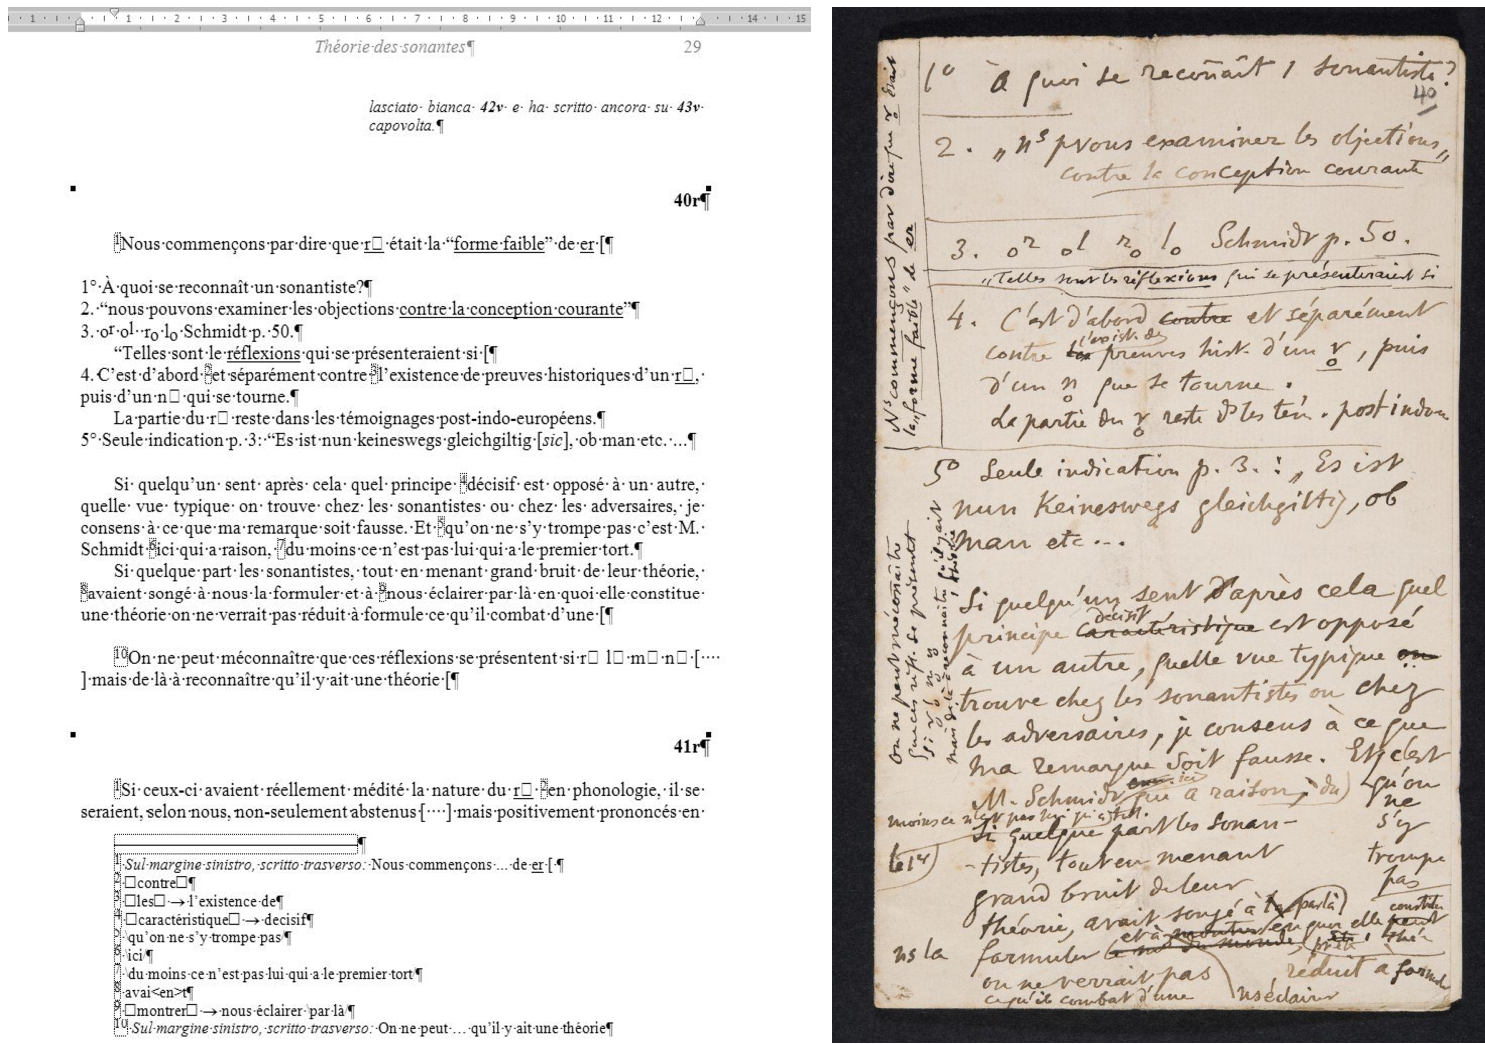
\includegraphics[width=.9\textwidth]{imgs/SaussureTrascrizione.pdf}
	\end{center}

\end{frame}


% frame 01
\begin{frame}
	\frametitle{Elementi di Codifica dei Caratteri}
	\framesubtitle{Definizioni}
	\addtocounter{nframe}{1}

	\begin{block}{Perché è importante la codifica dei caratteri}
		La codifica dei caratteri costituisce il grado zero (basso livello) della rappresentazione di testi su supporto digitale.
		\begin{center}
			\textit{Le codifiche dei caratteri sono la base di qualsiasi schema di codifica testuale}.
		\end{center}
	\end{block}

	\begin{block}{Rappresentazione digitale dei caratteri}
		I caratteri vengono rappresentati all’interno di un elaboratore mediante una sequenza di codici binari formati da opportune disposizioni di cifre composte da 0 e 1: 01100001 \textit{lettera a}
	\end{block}

\end{frame}



% frame 03
\begin{frame}
	\frametitle{Elementi di Codifica dei Caratteri}
	\framesubtitle{Definizioni}
	\addtocounter{nframe}{1}

	\begin{block}{Tabella Code Page ASCII 7 bit}
		%immagine di esempio Code Page ASCII (cp1252)
		\begin{center}
			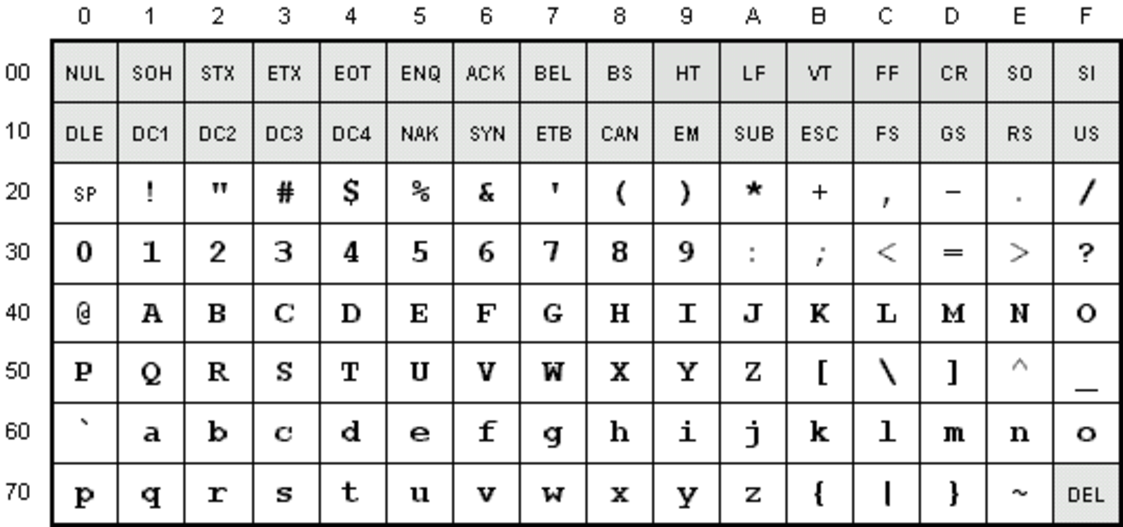
\includegraphics[width=.9\textwidth]{imgs/ascii-67.pdf}
		\end{center}

	\end{block}
	%\hline
	\begin{tiny}
		\begin{center}
			7 bit = 128 possibili caratteri; 32 caratteri di controllo; 96 caratteri effettivi
		\end{center}

	\end{tiny}

\end{frame}

% frame 0
\begin{frame}
	\frametitle{Elementi di Codifica dei Caratteri}
	\framesubtitle{Esempio codifica binaria}
	\addtocounter{nframe}{1}

	\begin{block}{codifica \textit{ciao mondo!} 7 bit ASCII}
		\begin{center}
			\textsc{6369 616f 206d 6f6e 646f 210a}
		\end{center}
	\end{block}

	\begin{block}{codifica \textit{ciao è mondo!} 8 bit ASCII}
		\begin{center}
			\textmd{6369 616f 20\textbf{e8} 206d 6f6e 646f 210a       }
		\end{center}
	\end{block}

	\begin{block}{codifica \textbf{ciao è mondo!} UNICODE UTF-8}
		\begin{center}
			6369 616f 20\textbf{c3 a8}20 6d6f 6e64 6f21 0a
		\end{center}
	\end{block}

\end{frame}

% frame 02
\begin{frame}
	\frametitle{Elementi di Codifica dei Caratteri}
	\framesubtitle{Definizioni}
	\addtocounter{nframe}{1}

	% \begin{block}{Character set, Code Set}
	%  - Character set
	%  - Code Set
	%  - Character encoding
	%  - Tabella del Code page
	% \end{block}

	\begin{description}
		\item [Character set] Per le discipline che studiano i sistemi di scrittura e l'analisi del linguaggio naturale, un insieme di caratteri astratti è detto Character set (unità alfabetiche). Astratto perché non riguarda la rappresentazione materiale della forma sul supporto, ma è relativo alla forma mentale, fatta di simboli di codifica (referenti).
		\item [Coded Char Set] Per poter trattare un insieme di unità alfabetiche in formato digitale bisogna assegnare a ciascun carattere un numero intero non negativo detto code point.
		
	\end{description}

\end{frame}

% frame 02b
\begin{frame}
	\frametitle{Elementi di Codifica dei Caratteri}
	\framesubtitle{Definizioni}
	\addtocounter{nframe}{1}

	% \begin{block}{Character set, Code Set}
	%  - Character set
	%  - Code Set
	%  - Character encoding
	%  - Tabella del Code page
	% \end{block}

	\begin{description}
		\item [Character encoding]  Il fine ultimo della codifica è quello di rappresentare una sequenza di caratteri in una sequenza di byte. La codifica di un carattere utilizza uno ``encoding schema'' che a sua volta mappa o trasforma ciascun code point in una sequenza di byte e quindi in ultima istanza in una sequenza di bit. 
		\item [Tabella del code page] Generalmente i code points sono espressi attraverso un sistema numerico esadecimale e disposti in una tabella di associazione.
	\end{description}

\end{frame}

% frame 02c
\begin{frame}
	\frametitle{Elementi di Codifica dei Caratteri}
	\framesubtitle{In sintesi}
	\addtocounter{nframe}{1}


	\begin{block}{Codifica dei caratteri}
		Quindi trasformare una sequenza di caratteri appartenenti ad un char set in una sequenza di byte (bit) significa prima di tutto trasformare/mappare ciascun carattere nel proprio corrispettivo code point e successivamente codificare/serializzare questo code point nella relativa sequenza di byte (bit).
	\end{block}

\end{frame}


% frame 0
\begin{frame}
	\frametitle{Elementi di Codifica dei Caratteri}
	\framesubtitle{Complessità e rappresentazione}
	\addtocounter{nframe}{1}

	\begin{block}{Complessità di rappresentazione universale dei caratteri}
		Se si considerano tutti i possibili alfabeti del mondo e le molteplici esigenze poste dalla scrittura delle fonti manoscritte antiche e medievali, ci si accorge che la realizzazione di un sistema universale per la codifica dei caratteri è un progetto molto complesso con svariate sfide da affrontare.
	\end{block}

\end{frame}

% frame 0
\begin{frame}
	\frametitle{Complessità e rappresentazione di Codifica dei Caratteri}
	\framesubtitle{Un Esempio}
	\addtocounter{nframe}{1}

	\begin{center}
		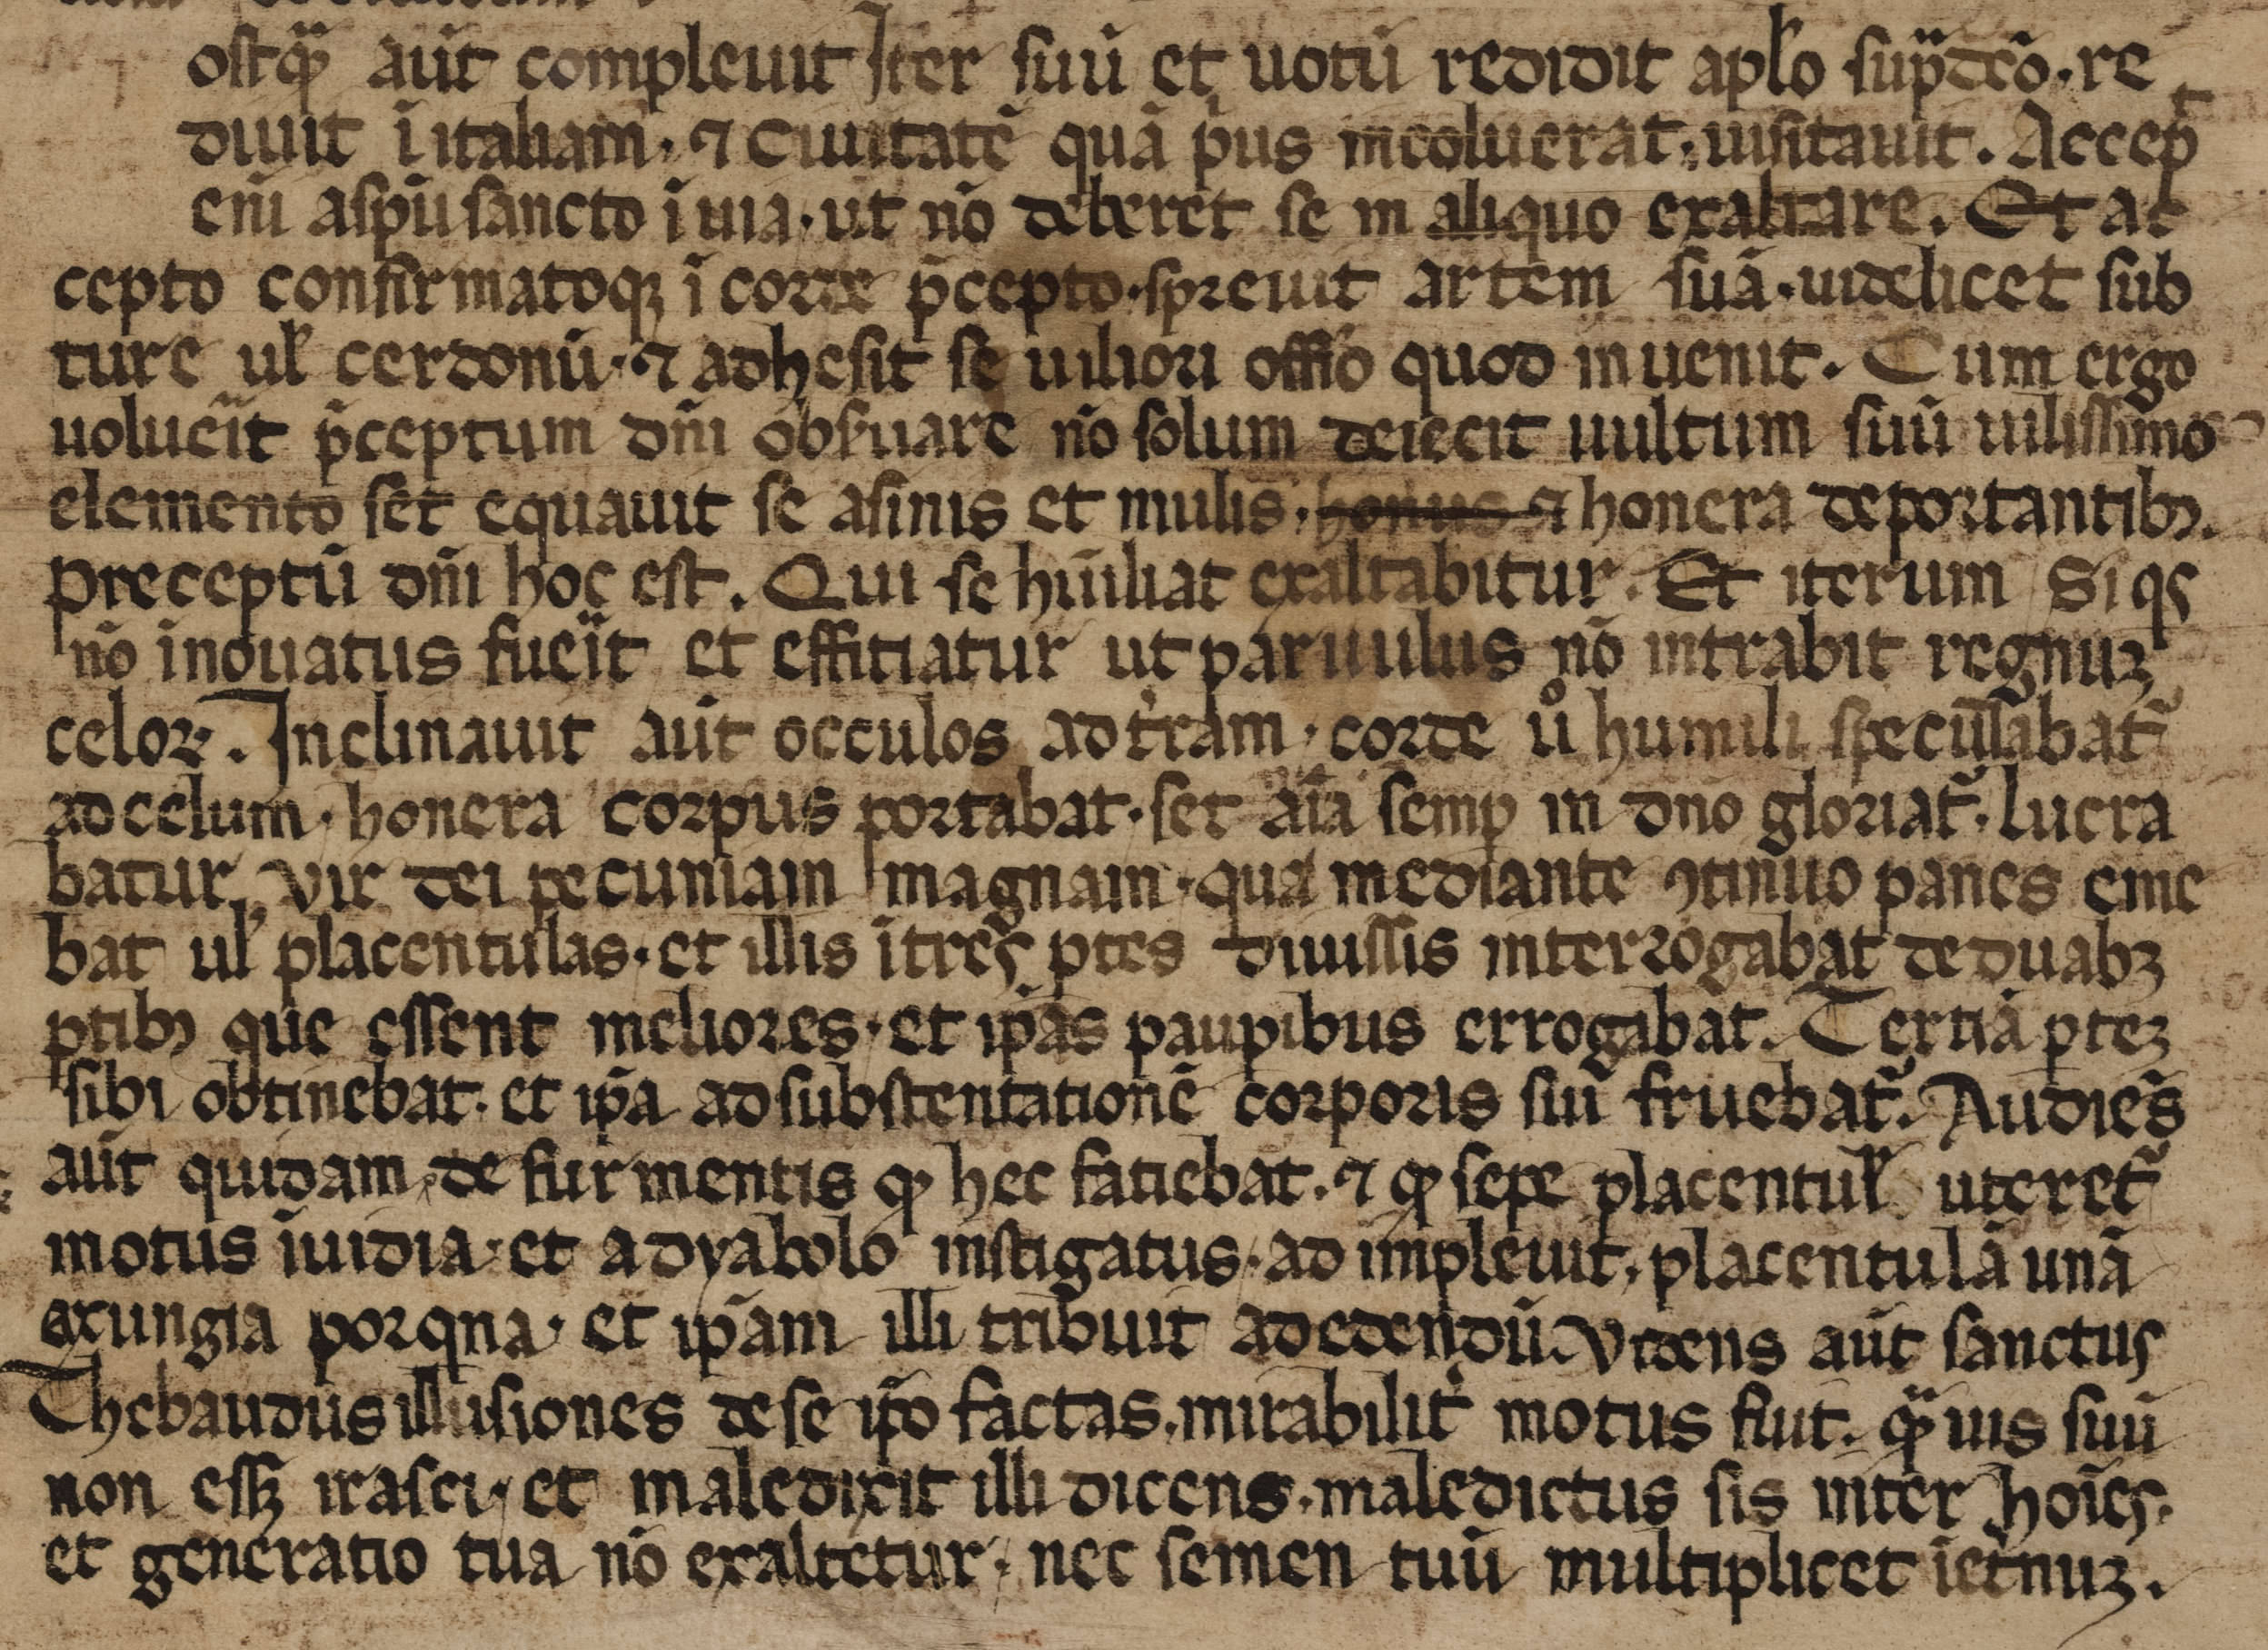
\includegraphics[width=.9\textwidth]{imgs/SnippetRotulo.jpg}
	\end{center}

\end{frame}

% frame 0
\begin{frame}
	\frametitle{Complessità e rappresentazione di Codifica dei Caratteri}
	\framesubtitle{Un Esempio}
	\addtocounter{nframe}{1}

	\begin{center}
		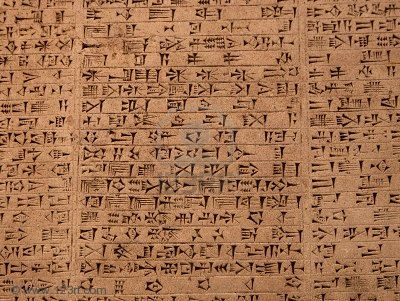
\includegraphics[width=.9\textwidth]{imgs/tavolettaArgilla.jpg}
	\end{center}

\end{frame}


\begin{frame}
	\frametitle{Elementi di Codifica dei Caratteri}
	\framesubtitle{Unicode}
	\addtocounter{nframe}{1}

	\begin{block}{Complessità di rappresentazione universale}
		Ad oggi, lo standard de facto per la codifica dei caratteri è lo UNICODE. Esso è in grado di codificare più di un milione di differenti unità alfabetiche, segni di interpunzione e diacritici, appartenenti a centinaia di diverse lingue.
	\end{block}

	\begin{block}{Complessità di rappresentazione universale}
		%(1.114.111)
		Unicode assegna i propri code point in un range che va da $0x0$ a $0x10FFFF$. In Unicode il code point viene  indicato con una ``U'' seguita da un segno ``+'' seguito a sua volta dall'esadecimale con padding del codice (es: U+0041 lettera a).
	\end{block}

\end{frame}

\begin{frame}
	\frametitle{Elementi di Codifica dei Caratteri}
	\framesubtitle{Unicode}
	\addtocounter{nframe}{1}

	\begin{block}{Unicode Transformation Format}
		Lo Unicode è un Coded Char Set e per essere concretamente serializzato su un supporto elettronico deve essere trasformato attraverso qualche tipo di schema di codifica.
		L'UTF (Unicode Transformation Format) mappa i code point Unicode in sequenze di byte (bit).
	\end{block}

	\begin{block}{UTF standards}
		Esistono tre tipi di schemi di codifica che vanno sotto il nome di UTF, ciascuno è identificato dal minimo numero di bit necessario a codificare ciascun code point: UTF-8; UTF-16; UTF-32. 
	\end{block}

\end{frame}



\section{Codifica dei Testi}
% riprendere qualcosa dalle slide Fiormonte Ciotti (Introduzione alla codifica XML per i testi umanistici)

% Il computer si è dimostrato un potente strumento per redigere, conservare, diffondere, analizzare i testi.
% % dalla slide vitali
% The ecosystem of text
% • Editing
% • Validating
% • Printing & displaying
% • Transforming and converting
% • Annotating
% – Annotating annotations
% • Searching
% • ... 



% detta difficile: “riconoscere un fenomeno dato come il token di un dato type presuppone alcune ipotesi sul contesto espressivo e sul co-testo discorsivo” (Eco)

% La codifica elettronica dei testi ha rappresentato uno dei temi fondamentali della riflessione e della sperimentazione nel dominio dell’Informatica umanistica.

% ad oggi la soluzione considerata ottimale per una corretta rappresentazione del testo è l'adozione dei markup language descrittivi basati su XML


\begin{frame}
	\frametitle{Rappresentazione digitale dei testi}
	\framesubtitle{basso e alto livello di codifica}
	\addtocounter{nframe}{1}

	\begin{block}{Codificare un testo}
		La codifica dei caratteri evidentemente non esaurisce i problemi per una opportuna rappresentazione delle caratteristiche interne ed esterne di un testo.
    \end{block}
    
    \begin{block}{Codificare un testo}
		Difatti la codifica del testo è una questione molto più complessa di una semplice riproduzione meccanica di un dato.
	\end{block}


\end{frame}


\begin{frame}
	\frametitle{Rappresentazione digitale dei testi}
	\framesubtitle{basso e alto livello di codifica}
	\addtocounter{nframe}{1}

	\begin{block}{Rappresentare un testo}
		
			La rappresentazione digitale di un testo è una operazione intrinsecamente assai difficile perché coinvolge una pletora di aspetti, a varie dimensioni, a varie granularità e a vari livelli di astrazione sia teorici, sia metodologici, sia tecnologici e sia pratici.
		
	\end{block}

\end{frame}

\begin{frame}
	\frametitle{Rappresentazione digitale dei testi}
	\framesubtitle{basso e alto livello di codifica}
	\addtocounter{nframe}{1}

	\begin{block}{Rappresentare un testo}
		\textbf{
			Prima di poter fare qualsiasi ipotesi su come compiere una codifica di un testo e su come rappresentarlo digitalmente, bisogna stabilire cosa si intende per testo.
		}
	\end{block}

\end{frame}


\begin{frame}
	\frametitle{Rappresentazione digitale dei testi}
	\framesubtitle{Modello dati di un testo}
	\addtocounter{nframe}{1}

	\begin{block}{Un testo non ha una struttura rigida, predefinita: }
		\begin{itemize}

			\item Non è rappresentabile solo come un insieme di record di un archivio elettronico.
			\item Non è rappresentabile solo come un insieme di tabelle di una banca dati.
			\item Non è rappresentabile solo come un albero o un insieme di sotto-alberi
			\item Non è rappresentabile solo come un grafo o come un insieme di sotto grafi

		\end{itemize}

	\end{block}

\end{frame}

\begin{frame}
	\frametitle{Molteplici modelli per diverse esigenze}
	\framesubtitle{Strutture dato e testo}
	\addtocounter{nframe}{1}

	\begin{block}{La rappresentazione di un testo}
		\begin{itemize}
			 %mia slide sulle possibili rappresentazioni del testo
			\item modello lineare: sequenza di dati non strutturati
			\item modello  a record: enumerazione delle proprietà
			\item modello tabulare: insieme di dati omogenei
			\item modello ad albero: gerarchie di dati e insiemi di dati
			\item modello grafo: rete di strutture informative interconnesse tra loro
        \end{itemize}
        
	\end{block}
\end{frame}



\begin{frame}
	\frametitle{Elementi di Codifica del testo}
	\framesubtitle{Formalismi}
	\addtocounter{nframe}{1}

	\begin{block}{Formati di rappresentazione}
		\begin{center}
			Un formato è un insieme di regole e convenzioni formali per rappresentare un insieme di dati, nel nostro caso un testo.
		\end{center}

	\end{block}

	\begin{block}{Importanza dei formati}
		\begin{center}
			Seppur isomorfi la scelta dei formati condiziona molto l'efficienza delle operazioni e l'efficacia delle dichiarazioni.
		\end{center}

	\end{block}


\end{frame}

%\begin{frame}
%    \frametitle{Elementi di Codifica del testo}
%    \framesubtitle{lista di formati}
%    \addtocounter{nframe}{1}
%   
%    \begin{block}{Formati dato}
%Data structures – CSV and tabular data
%– JSON
%– RDF
%Plain text formats – Plain text
%– TeX, LaTeX, etc.
%– Markdown, CommonMark and wiki syntaxes
%Markup formats
%– HTML, HTML5
%– XML
%– HTML5+ Embedded annotations (e.g., HTML5 + RDFa)
%– Markup spinoffs for overlapping (e.g. LMNL, TexMECS, etc.) 
%
%    \end{block}

% \begin{block}{Riferimenti TEI}
%     Capitolo sul character encoding e modulo Ganji 
% \end{block}

%\end{frame}

\begin{frame}
	\frametitle{Elementi di Codifica del testo}
	\framesubtitle{Tabella Formalismi}
	\addtocounter{nframe}{1}

	\begin{block}{Formalismi}
		\begin{center}
			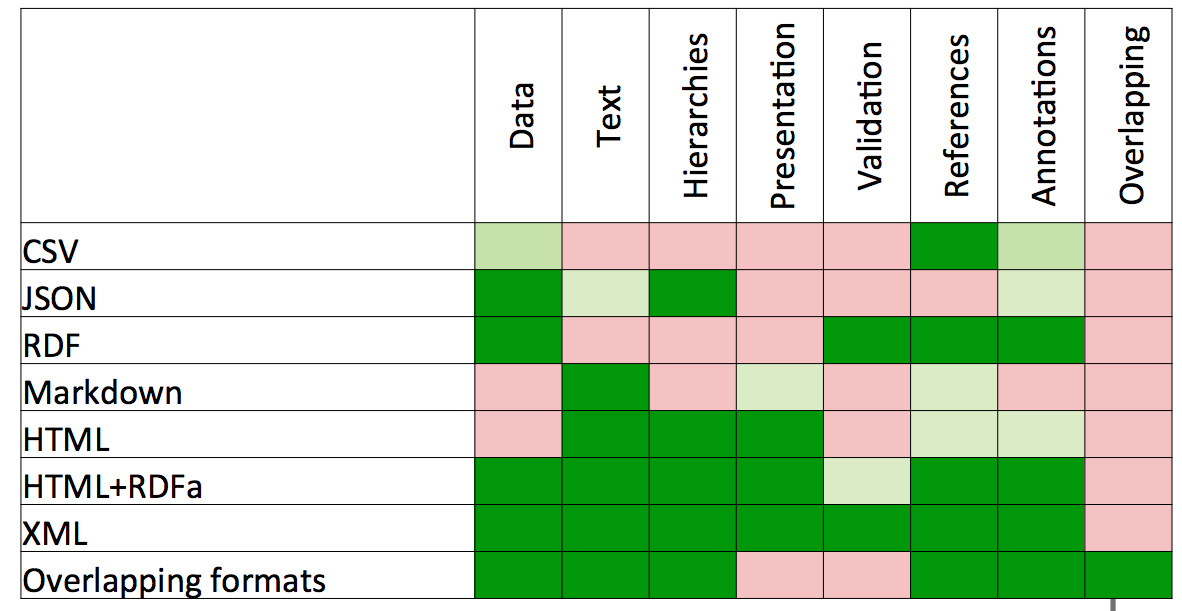
\includegraphics[width=.9\textwidth]{imgs/TabellaFormalismiCodificaTesto.png}
		\end{center}
	\end{block}
	courtesy of \textit{Fabio Vitali}

\end{frame}


\begin{frame}
	\frametitle{Elementi di Codifica del testo}
	\framesubtitle{Varietà di rappresentazione}
	\addtocounter{nframe}{1}

	
		\begin{center}
			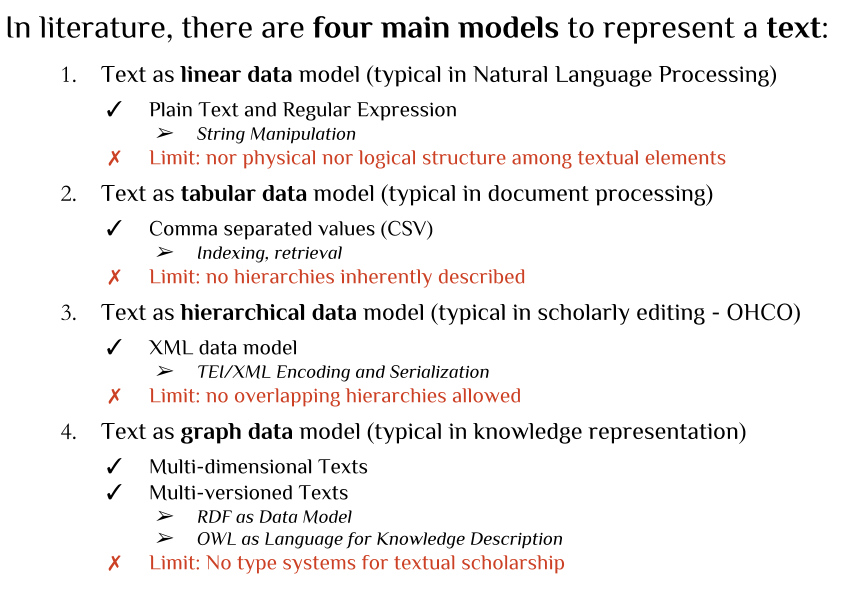
\includegraphics[width=.9\textwidth]{imgs/dataModels-slide.png}
		\end{center}
	
	
\end{frame}

\begin{frame}
	\frametitle{Elementi di Codifica del testo}
	\framesubtitle{Esempio di codifica del testo utilizzando CSV}
	\addtocounter{nframe}{1}

		
			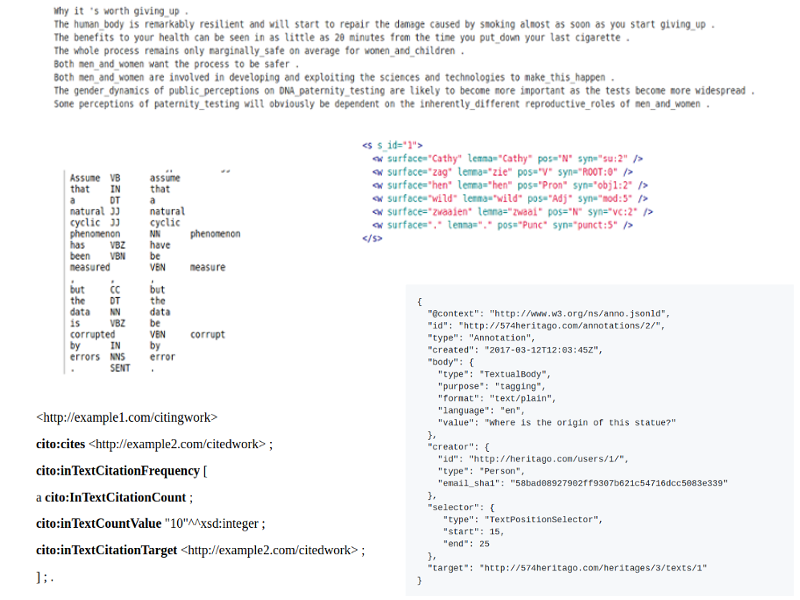
\includegraphics[width=1.1\textwidth]{imgs/VariRappresentazioniTesto.png}
		
	
\end{frame}



\begin{frame}
	\frametitle{Elementi di Codifica del testo}
	\framesubtitle{Formalismi}
	\addtocounter{nframe}{1}

	\begin{block}{Formati come formalismi}
		\begin{center}
			Data l'importanza metodologica il formato del dato diviene un vero e proprio formalismo, si parla cioè di linguaggi di codifica in quanto questi sistemi si basano su un insieme di istruzioni rigorose di codifica.
		\end{center}

	\end{block}

\end{frame}



\begin{frame}
	\frametitle{Elementi di Codifica del testo}
	\framesubtitle{Formalismi}
	\addtocounter{nframe}{1}

	\begin{block}{Formati e formalismi di codifica}

		Quindi ogni pezzo di informazione aggiunta ad un testo grezzo attraverso l'inserimento di dati metatestuali (markup, annotazione, codifica), constituisce il risultato di una analisi e di una interpretazione che è stata condotta (da un umano o da una macchina) al fine di esplicitare e rappresentare nel modo più accurato e completo possibile le informazioni da veicolare attraverso il formato digitale prescelto (anche in modo incrementale).


	\end{block}

\end{frame}





% % altra slide Vitali
% • Text has characters, including punctuation
% – We all (sort of) agree on this
% • Texts is ordered
% – In ``To be or not to be'', it is important that ``To be''
% comes before ``not to be''
% • Text has structure
% • Text has presentation
% • Text has grammar
% • Texts has semantics
% • Text has variants
% • Text has a lot of things that can be said about it 


\section{Ecosistema XML}
% importanza dell'XML
 %% leggere capitolo 1 del libro XML schema complete reference 2003 (cliff, etc..)
% importanza della definizione di uno schema XML
% importanza della definizione di trasformate XSL e manipolazione del DOM

% Da slide Vitali:
XML allows to create markup languages that are
readable, generic, structured, hierarchical.
– Data: no problem
– Hierarchical data: no problem
– Text: no problem
– Presentation of data: after transformation via XSLT
– Hierarchical text: no problem
– Validation: no problem
– References: no problem
– Annotations: as attributes or ad hoc sections of the
document 

% Da Slide Chiara
% XPath: XML Path Language
% XSL: eXtensible Stylesheet Language
% XSL-T: eXtensible Stylesheet Lang. – Transformations
% XSL-FO: eXtensible Stylesheet Lang. – Formatting Objects
% XQuery: XML Query language for XML Databases
% XInclude: XML inclusion language
% RelaxNG: Regular Expression Language for XML (New Generation)


\section{Conclusioni}
% strumenti per l'editing XML
%% editor di testi plain text
%% Oxygen
%% VSCode
%% editiXML


% bibliografia di riferimento
%% Ciotti
%% Burnard
%% TEI guide lines
%% Pierazzo
%% Slide
%% XML visual
%% XSL XPATH
%% XSD DTD RELAXNG

% esercitazioni e approfondimenti

% modalità di esame
% progetto
% materiali e slide del corso
%% github


\section{Bibliografia}
%bibliografia
\begin{frame}
    \frametitle{References}
    \addtocounter{nframe}{1}
    \begin{thebibliography}{10}

        \setbeamertemplate{bibliography item}[paper]
        \tiny\bibitem{ciotti2011} Ciotti 2011

        \setbeamertemplate{bibliography item}[online]
        \tiny\bibitem{CCwikiBY2014} CC Wiki \textit{Best practices for attribution}, CC Wiki 2014, \url{https://wiki.creativecommons.org/wiki/Best\_practices\_for\_attribution}

    \end{thebibliography}

\end{frame}


\end{document}